\subsection{Seeds Data}
\textit{written by B.L.}\\

This data set has been used in the work of \cite{charytanowicz2010complete}. The data comprises information on different features of wheat kernels. There are seven species with a total of about 20 varieties of which three can be found in the data: Kama, Rosa and Canadian wheat. The kernels for which data was collected were selected randomly. They were then examined through X-ray imaging. A software called \textit{GRAINS} for this specific application \cite{strumillo1999computer} was used to extract the features for each observation:

\begin{multicols}{2}
\begin{itemize}
\item area $A$
\item perimeter $P$
\item compactness $C = 4 \pi A/P^{2}$
\item length (along groove)
\item width
\item asymmetry coefficient
\item length of kernel groove
\item label
\end{itemize}
\end{multicols}

A brief look into the data set confirms this.

\begin{table}[H]
\begin{center}
\resizebox{\textwidth}{!}{%
\begin{tabular}{lrrrrrrrl}
{} &   Area &  Perimeter &  Compactness &  Length &  Width &  Asymmetry &  Groove & Label \\ \hline
1 &  15.26 &      14.84 &        0.871 &   5.763 &  3.312 &            2.221 &          5.220 &  1 \\
2 &  14.88 &      14.57 &        0.881 &   5.554 &  3.333 &            1.018 &          4.956 &  1 \\
3 &  14.29 &      14.09 &        0.905 &   5.291 &  3.337 &            2.699 &          4.825 &  1 \\
4 &  13.84 &      13.94 &        0.896 &   5.324 &  3.379 &            2.259 &          4.805 &  1 \\
5 &  16.14 &      14.99 &        0.903 &   5.658 &  3.562 &            1.355 &          5.175 &  1 \\
\end{tabular}
}
\end{center}
\caption{Seeds Data Set First Observations}
\label{tab:seeds_key_facts}
\end{table}

\begin{figure}[H]
\caption{Seeds pairplot WIP}
%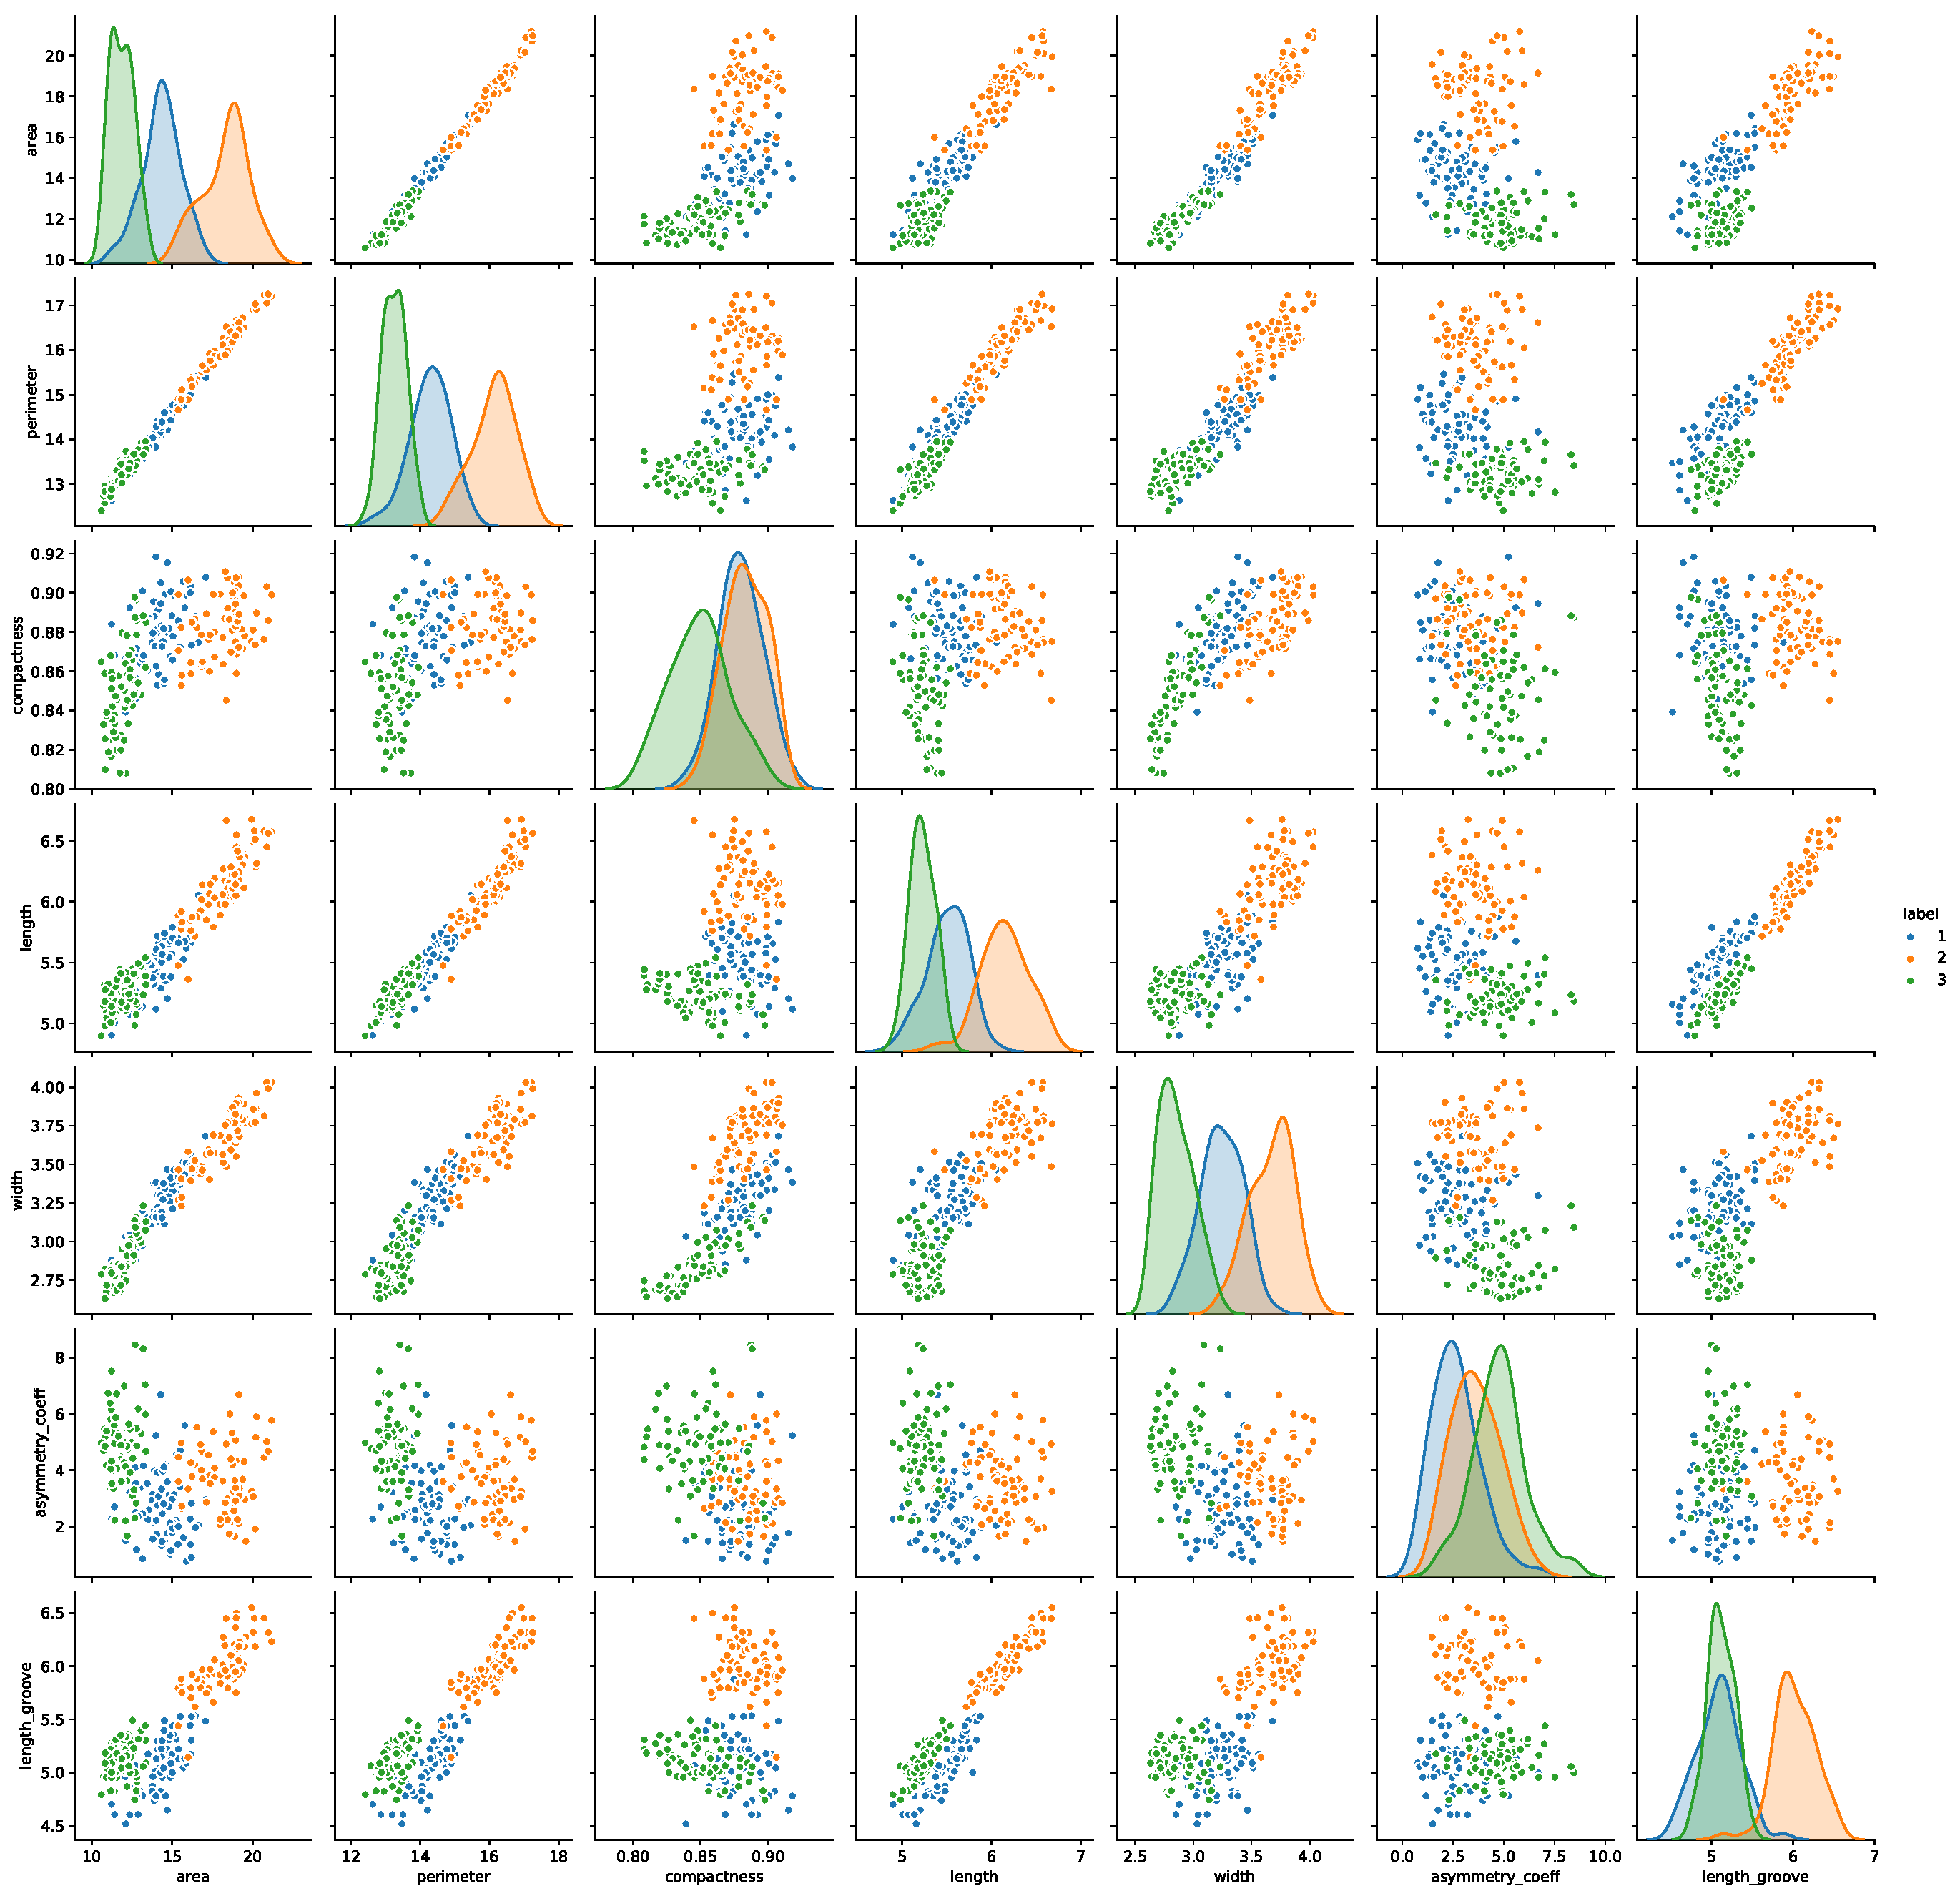
\includepdf[pages=-,scale=.4]{images/seeds_pairplot.pdf}
\begin{center}
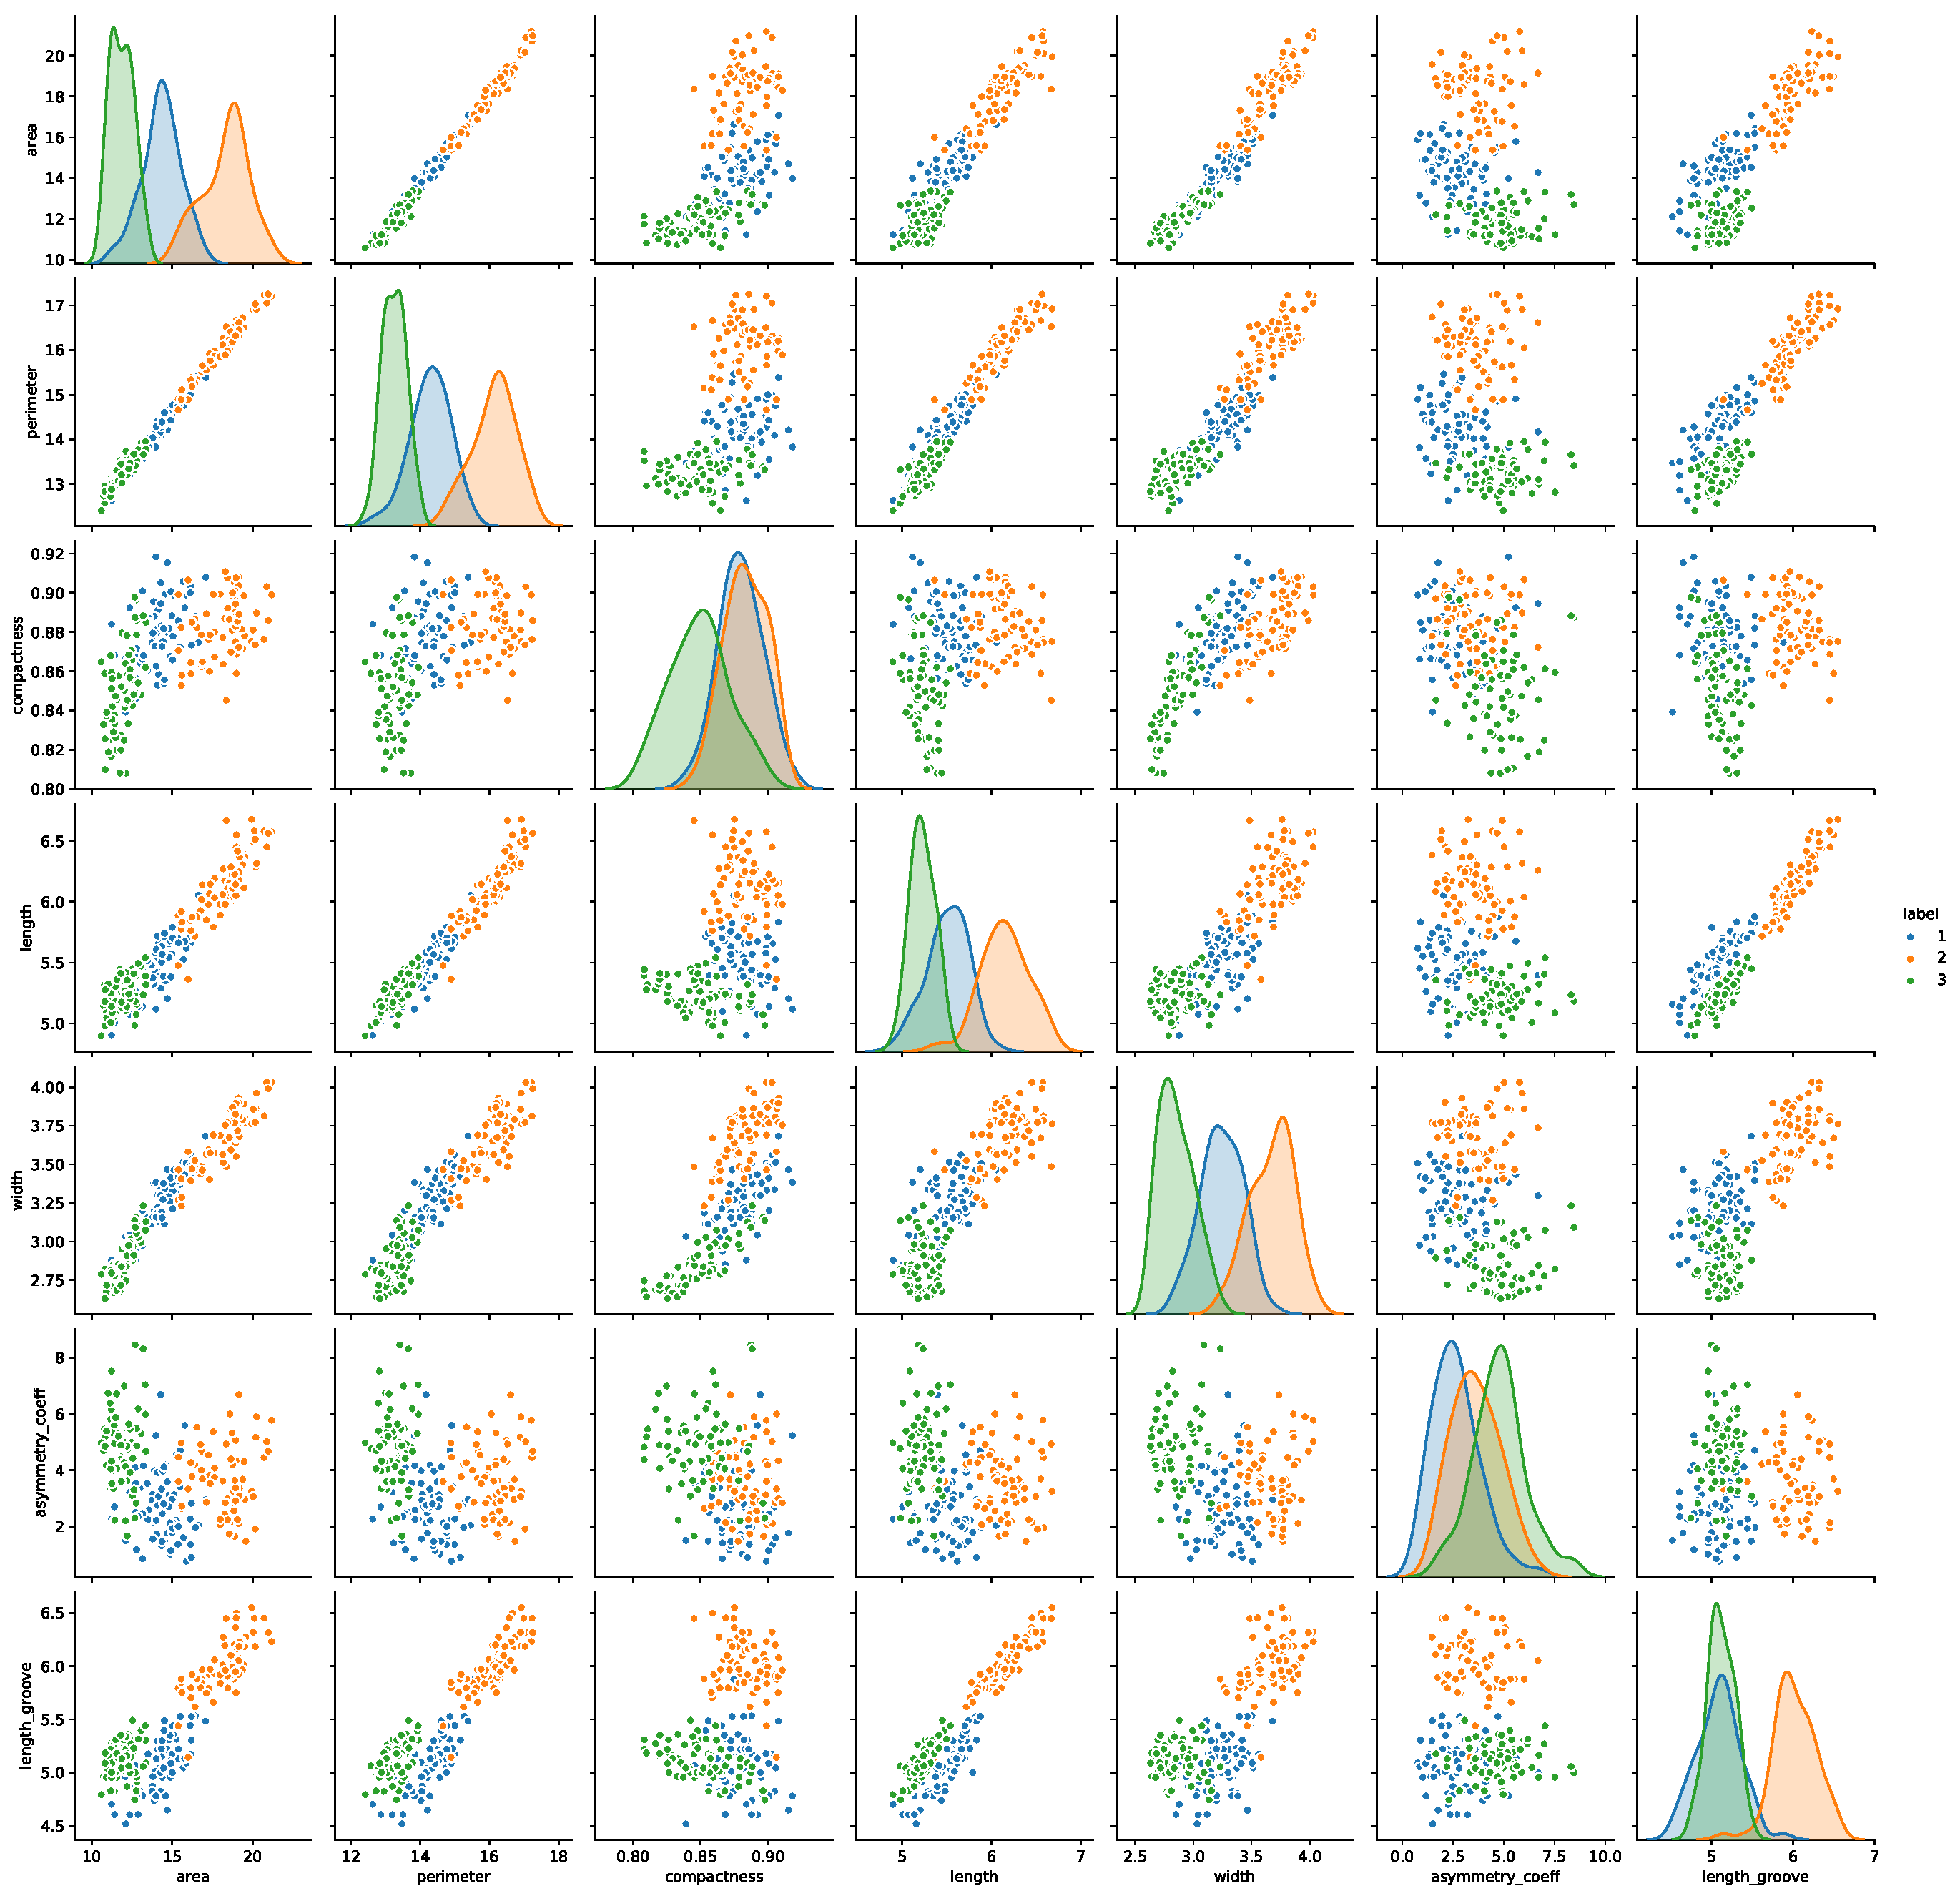
\includegraphics[width=0.9\textwidth]{images/seeds_pairplot.pdf}
\end{center}
\label{fig:seeds_pairplot}
\end{figure}

\vspace{-0.5cm}
A few things can be noted: compactness is linearly dependent on two other features in the data set, calling into question what value this information can bring to a clustering method. Furthermore the area is not computed from other measurements, but is correlated with width and length and the perimeter. These relationships among others can be seen in figure \ref{fig:seeds_pairplot}. Note that these plots have been colored according to their original labels. Density plots on the diagonal for example already show distinct characteristics for the different varieties of kernels for certain features. 

Some key insights on the data set as a whole can be found in table \ref{tab:seeds_key_facts} with information on the observation count, mean, standard deviation (std), minimum and maximum as well as 25, 50 and 75\% quantiles as rows for each feature in columns. There are a total of 210 observations which is on the lower end for clustering applications. The data is balanced at 70 observations for each kernel variety. There is no missing data in any of the features.

\begin{table}[H]
\begin{center}
\resizebox{\textwidth}{!}{%
\begin{tabular}{lrrrrrrr}
%\toprule
{} & Area &  Perimeter & Compactness & Length & Width & Asymmetry &  Groove \\
\hline
Count &  210 &    210 &      210 &  210 &  210 &          210 &        210 \\
Mean  &   14.848 &     14.559 &        0.871 &    5.629 &    3.259 &            3.700 &          5.408 \\
Std   &    2.910 &      1.306 &        0.024 &    0.443 &    0.378 &            1.504 &          0.491 \\
Min   &   10.590 &     12.410 &        0.808 &    4.899 &    2.630 &            0.765 &          4.519 \\
25\%   &   12.270 &     13.450 &        0.857 &    5.262 &    2.944 &            2.561 &          5.045 \\
50\%   &   14.355 &     14.320 &        0.873 &    5.524 &    3.237 &            3.599 &          5.223 \\
75\%   &   17.305 &     15.715 &        0.888 &    5.980 &    3.562 &            4.769 &          5.877 \\
Max   &   21.180 &     17.250 &        0.918 &    6.675 &    4.033 &            8.456 &          6.550 \\
%\bottomrule
\end{tabular}
}
\end{center}
\caption{Seeds Data Set Statistics Summary}
\label{tab:seeds_key_facts}
\end{table}

A few more things can be noted here: Rosa wheat kernels exhibit a mean area more than one standard deviation above the mean area for the entire data. Similarly, Canadian wheat kernels have a mean asymmetry coefficient far beyond one standard deviation above the overall mean. For each variety of wheat a normality test \cite{d1973tests} has shown that the hypothesis of normality cannot be rejected at a 99\% level for most features. This might bode well for at least K-Means clustering.


For the clustering step of course the labels are removed from the data (this data set was included despite not being the typical application of clustering in part because it can serve as a sort of "control" for the clustering methods when looking at evaluation and conclusions).



